% Source-coordinate reconstruction. Edit named defaults or copy this entire composition.
\studiodeclarefield{graphic-1}{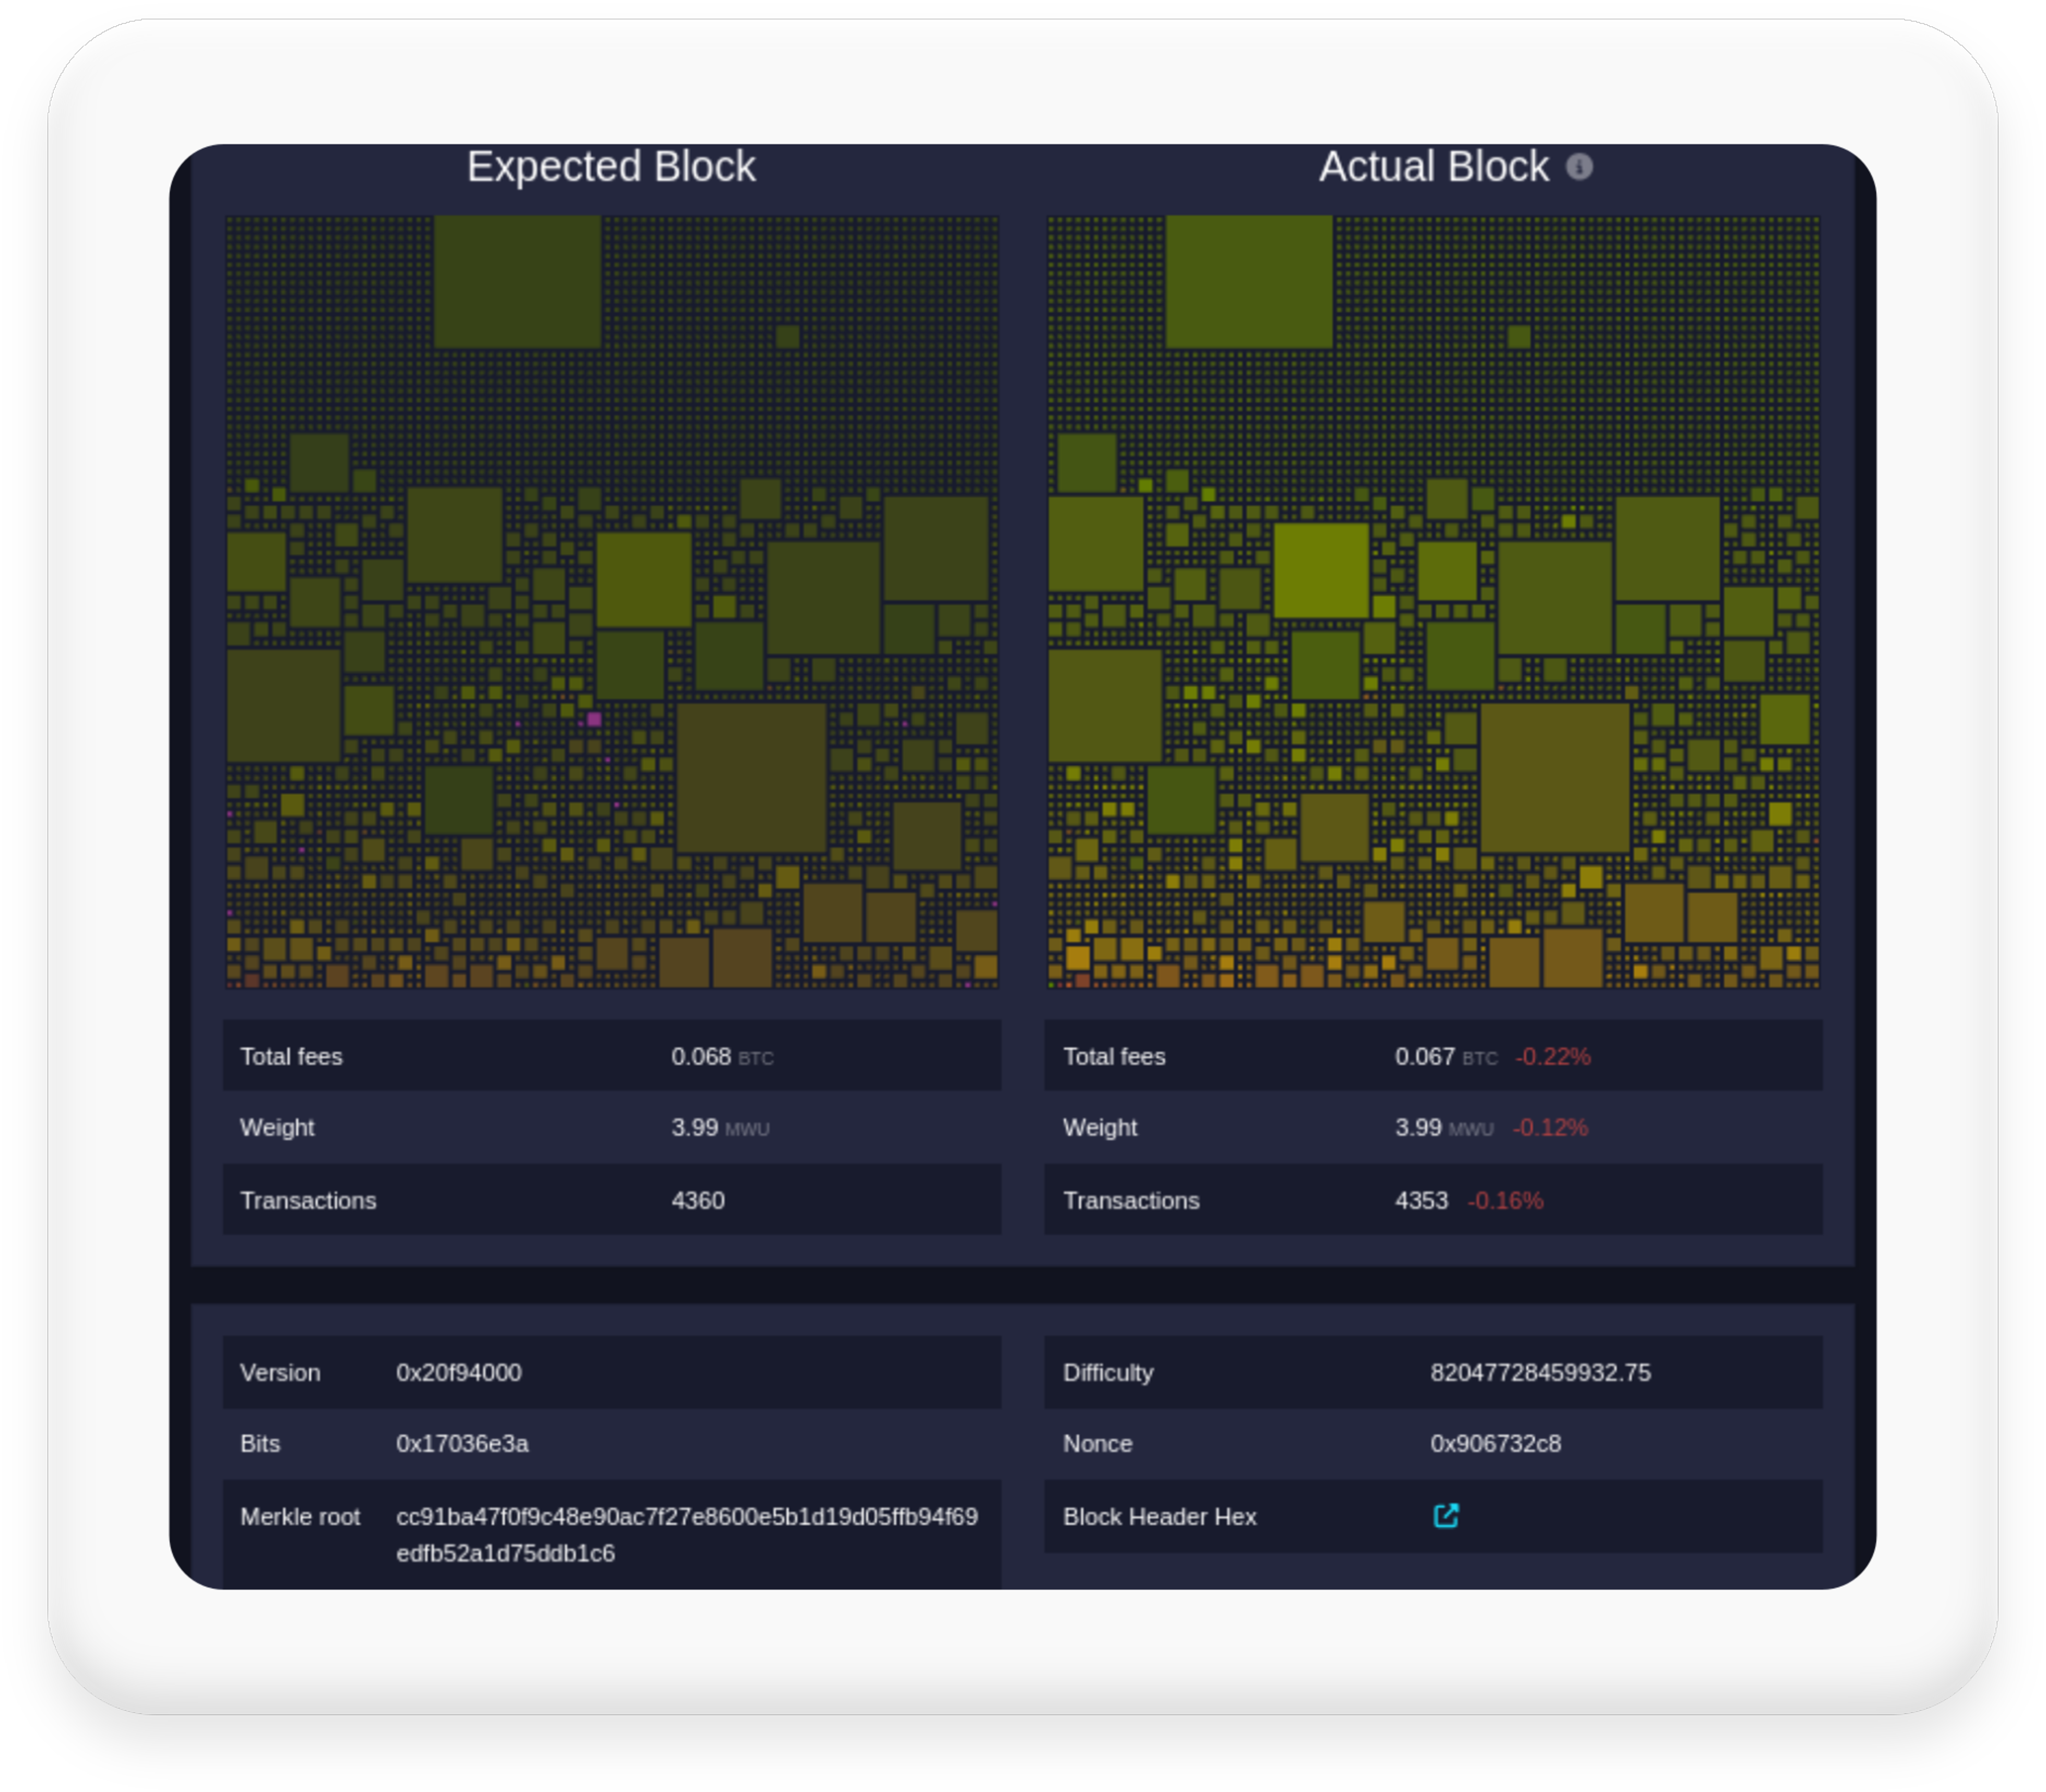
\includegraphics[width=1881\studiounit]{images/studio/collection/figma-0530-part-01.pdf}}
\studiodeclarefield{text-1}{The hash must fall below\\a target threshold (Bits)}
\studiodeclarefield{text-2}{Retarget every 2016\\blocks (about 2 weeks)}
\studiodeclarefield{text-3}{Indicates the difficulty\\of Proof-of-Work}
\studiodeclarefield{title}{Difficulty}
\studioapplyfields
\studiomeasuredcanvas{3556}{2000}{screenshot-callout}{studio-paper}{
\studiographfield{graphic-1}{1507}{203}{1881}{1648}{}{}
\studiomeasuredtext{text-1}{347.383}{1046.85}{1088.03}{207.975}{75.16}{87.1856}{\color{bitpolito}}{\studiofield{text-1}}
\studiomeasuredtext{text-2}{349.492}{1337.7}{816.109}{207.993}{76.4}{88.624}{\color{bitpolito}}{\studiofield{text-2}}
\path[fill=bitpolito,draw=none,line width=1\studiounit] (269.5,1075.5) circle[radius=19.5\studiounit];
\path[fill=bitpolito,draw=none,line width=1\studiounit] (269.5,1366.5) circle[radius=19.5\studiounit];
\studiomeasuredtext{text-3}{347.344}{754.953}{1571.39}{195.804}{76.2493}{88.4492}{\color{bitpolito}}{\studiofield{text-3}}
\path[fill=bitpolito,draw=none,line width=1\studiounit,rounded corners=8\studiounit] (262,1123) rectangle (278,1319);
\path[fill=bitpolito,draw=none,line width=1\studiounit] (269.5,784.5) circle[radius=19.5\studiounit];
\path[fill=bitpolito,draw=none,line width=1\studiounit,rounded corners=8\studiounit] (262,832) rectangle (278,1028);
\studiomeasuredtext{title}{257.441}{518.047}{545.555}{170.484}{114.375}{132.675}{\color{bitpolito}\bfseries}{\studiofield{title}}
}
